\documentclass[9pt]{beamer}
\usetheme{Madrid}
\usefonttheme{serif}

\usepackage{fontspec}
% надёжный шрифт с кириллицей (работает в Overleaf)
\setmainfont{Libertinus Serif}[Ligatures=TeX]
\setsansfont{Libertinus Sans}[Ligatures=TeX]
\newfontfamily\cyrillicfont{Libertinus Serif}
\newfontfamily\cyrillicfontsf{Libertinus Sans}
\usepackage{polyglossia}
\setmainlanguage{russian}
\setotherlanguage{english}

\usepackage{amsmath}
\usepackage{amsfonts}
\usepackage{amssymb}
\usepackage{graphicx}
\usepackage{microtype}

\usepackage{tabularx}
\usepackage{booktabs}

\usepackage{xcolor}
\usepackage{pifont}
\usepackage{tikz}
\newcommand{\plus}{\tikz[baseline=(X.base)] \node[fill=green!65!black, rounded corners=2pt, inner sep=2pt] (X) {\color{white}\ding{51}};}
\newcommand{\minus}{\tikz[baseline=(X.base)] \node[fill=red!70!black,   rounded corners=2pt, inner sep=2pt] (X) {\color{white}\ding{55}};}

\DeclareMathOperator{\sen}{sen}
% \DeclareMathOperator{\tg}{tg}

\setbeamertemplate{caption}[numbered]

% --- Информация о презентации ---
\author[Автор]{Чиняев Владимир Николаевич}
\title{Задача перехода в линейном приближении \\ (некомпланарный случай) \\ Расстояние между орбитами}
\newcommand{\coursename}{Введение в маневрирование КА}
\setbeamertemplate{navigation symbols}{} 
\institute[]{Московский физико технический институт} 
\date{7 октября 2025 г.} 

\bibliographystyle{apalike}

% --- Кастомная нижняя синяя полоска: курс слева, номер слайда справа ---
\setbeamertemplate{footline}{
  \leavevmode%
  \begin{beamercolorbox}[wd=\paperwidth,ht=2ex,dp=1ex]{palette primary}
    \hspace{0.4cm}\usebeamerfont{footline}\coursename\hfill\usebeamerfont{footline}\insertframenumber\hspace{0.4cm}
  \end{beamercolorbox}%
}

% Чтобы убрать лишние отступы в footer-шрифте (опционально)
\setbeamerfont{footline}{size=\small}

\begin{document}

\begin{frame}
\titlepage
\end{frame}

\begin{frame}{D-критерий}
Для того чтобы иметь возможность анализировать результаты работы алгоритмов маневрирования, необходимо научиться определять расстояния между парами орбит. В первую очередь рассмотрим невозмущённые кеплеровы орбиты \textemdash\ зафиксированные в пространстве эллипсы $\textbf{Э} = \left( a, e, i, \omega, \Omega \right)^T$, имеющие постоянные геометрические характеристики.

Метрику можно ввести бесконечным числом способов. Одна из первых таких попыток описана в работе Р. Б. Саузворта и Дж. С. Хокинса \cite{Southworth_Hawkins}. Они отмечают, что никакая мера близости орбит не определена априори. А потому, авторы искали простую, насколько это возможно, и выражающуюся в терминах орбитальных элементов, метрику. Для её построения они провели аналогию с пятимерным пространством, в котором введена ортогональная СК, и рассмотрели каждый орбитальный элемент как координату. Таким образом, любая орбита соответствует точке в этом пространстве и расстояние между двумя орбитами $\textbf{Э}_1$ и $\textbf{Э}_2$ может быть записано в виде:
\begin{equation*}
    D^2(\textbf{Э}_1, \textbf{Э}_2) = \sum_{j=1}^{5} c_j^2 [C_j(\textbf{Э}_1) - C_j(\textbf{Э}_2)]^2,
\label{D-crit_first}
\end{equation*}
где $C_j$, $j \in \{1, 2, 3, 4, 5\}$, \textemdash\ независимые функции кеплеровых элементов соответствующей орбиты; $c_j$, $j \in \{1, 2, 3, 4, 5\}$, \textemdash\ функции кеплеровых элементов орбит $\textbf{Э}_1$ и $\textbf{Э}_2$, которые определяют геометрию пространства. 
\end{frame}

\begin{frame}{Метрика Холшевникова}
К. В. Холшевников вводит пространство $\mathbf{E}$, элементами которого являются ориентированные кеплеровы эллипсы $E$. Пусть $Q(u)$ \textemdash\ это точка на эллипсе $E \in \mathbf{E}$, имеющая эксцентрическую аномалию $u$; $s(Q_1, Q_2)$ - это евклидово расстояние в $\mathbb{R}^3$. Теперь введём функцию $\rho$, зависящую от параметра $p \in [1, \infty]$ и отображающую $\mathbf{E} \times \mathbf{E}$ в множество неотрицателльных чисел:
\begin{equation*}
    \rho (p, E_1, E_2) = \min \biggl( \frac{1}{2\pi} \int s^p (Q_1(u), Q_2(u + v)) du \biggl)^{1/p}.
\label{distance_first}
\end{equation*}
Кроме того, в статье \cite{Kholshevnikov} представляются необходимые доказательства того, что метрика выше удовлетворяет всем аксиомам метрического пространства. 
\end{frame}

\begin{frame}{Метрика Холшевникова}
Введём несколько обозначений, которые понадобятся нам в дальнейшем. Радиус-вектор $\mathbf{r}$ точки на орбите $E$ может быть задан следующим выражением:
\begin{equation*}
   \frac{\mathbf{r}}{a} = \mathbf{P} (\cos u - e) + \mathbf{S} \sin u,
\end{equation*}
где $\mathbf{S} = \eta \mathbf{Q}$, $\eta = \sqrt{1 - e^2}$, и векторы $\mathbf{P}$ и $\mathbf{Q}$ имеют компоненты:
\begin{gather*}
    P_x = \cos \omega \cos \Omega - \cos i \sin \omega \sin \Omega, \\
    P_y = \cos \omega \sin \Omega + \cos i \sin \omega \cos \Omega, \quad
    P_z = \sin i \sin \omega, \\
    Q_x = -\sin \omega \cos \Omega - \cos i \cos \omega \sin \Omega, \\
    Q_y = -\sin \omega \sin \Omega + \cos i \cos \omega \cos \Omega, \quad
    Q_z = \sin i \cos \omega.
\end{gather*}
\end{frame}

\begin{frame}{Метрика Холшевникова}
Кроме того
\begin{gather*}
    \alpha = \frac{a}{a'}, \quad \alpha' = \frac{a'}{a}, \\
    4W_0 = 2(\alpha + \alpha') + \alpha e^2 + \alpha'^2 e'^2 - 4 \langle \mathbf{P}, \mathbf{P}' \rangle e e', \\
    2W_5 = - \langle \mathbf{P}, \mathbf{P}' \rangle, \quad 
    2W_6 = - \langle \mathbf{P}, \mathbf{S}' \rangle, \quad
    2W_7 = - \langle \mathbf{P}', \mathbf{S} \rangle, \quad
    2W_8 = - \langle \mathbf{S}, \mathbf{S}' \rangle,
\end{gather*}
где $\langle \cdot, \cdot \rangle$ \textemdash\ это скалярное произведение векторов. Тогда можно написать выражение для расстояния между двумя кеплеровыми орбитами $E_1$ и $E_2$ на пространстве $\mathbf{E}$ для $p = 2$:
\begin{equation*}
    \rho^2 (2, E_1, E_2) = 2aa' \biggl( W_0 - \sqrt{(W_5 + W_8)^2 + (W_6 - W_7)^2} \biggl).
\label{distance}
\end{equation*}
\end{frame}

\begin{frame}{D-критерий vs. метрика Холшевникова (1/2)}
\footnotesize
\setlength{\tabcolsep}{4pt}
\renewcommand{\arraystretch}{1.25}
\begin{tabularx}{\linewidth}{p{0.23\linewidth} X X}
\toprule
\textbf{Критерий} &
\textbf{Взвешенная сумма по элементам} &
\textbf{Метрика Холшевникова}
\\ \midrule
Геометрический смысл &
Абстрактная «евклидова» метрика в пространстве параметров; смысл зависит от весов и набора элементов. &
Геометрическое расстояние между эллипсами в $\mathbb{R}^3$, усреднённое по аномалии и минимизированное по фазе.
\\
Инвариантность к смене ИСК &
Не гарантирована (зависит от параметризации и нормировок). &
Да: строится на скалярных произведениях $\mathbf P,\mathbf Q$; зависит только от взаимной геометрии.
\\
Зависимость от линии апсид &
Сильная: разности $\omega,\Omega$ могут доминировать. &
Фазовый сдвиг $v$ «выравнивает» ориентацию; непрерывное поведение при $e\!\to\!0$.
\\
Сингулярности элементов &
Возникают при $e\!\to\!0$ и $i\!\to\!0$ (неопределённость $\omega,\Omega$). &
Отсутствуют: работают через $\mathbf P,\mathbf Q$ и $\eta=\sqrt{1-e^2}$.
\\
Физическая релевантность для манёвров &
Косвенная: близость параметров $\not\Rightarrow$ близость траекторий. &
Прямая: измеряет среднюю пространственную близость орбитальных кривых.
\\
Чувствительность к масштабам &
Сильно зависит от произвольных весов $c_j$ и единиц измерения. &
Естественное масштабирование через множитель $2aa'$.
\\ \bottomrule
\end{tabularx}
\end{frame}

\begin{frame}{D-критерий vs. метрика Холшевникова (2/2)}
\footnotesize
\setlength{\tabcolsep}{4pt}
\renewcommand{\arraystretch}{1.25}
\begin{tabularx}{\linewidth}{p{0.23\linewidth} X X}
\toprule
\textbf{Критерий} &
\textbf{Взвешенная сумма по элементам} &
\textbf{Метрика Холшевникова}
\\ \midrule
Метрические аксиомы (треугольник и т.д.) &
В общем случае не доказаны (часто эвристика). &
Доказанная метрика на пространстве эллипсов.
\\
Гладкость для градиентных методов &
Гладкая. &
Гладкая.
\\
Поведение на почти совпадающих орбитах &
Может переоценивать различия из-за угловых элементов. &
Даёт малое и физичное расстояние; устойчива к апсидальной расстройке.
\\
Численная сложность &
Минимальная (разности элементов + веса). &
Низкая: построить $\mathbf P,\mathbf Q$, скалярные произведения.
\\
Настраиваемость («рукоятки») &
Гибкая: выбор весов под задачу/данные. &
Фиксированная метрика.
\\
Интерпретируемость результата &
«Сколько и какие элементы различаются» — понятно, но не геометрично. &
«Средняя пространственная дистанция после лучшего фазового выравнивания» — прямая геометрия.
\\
Когда выбирать &
Быстрые эвристики, грубый отбор, когда важна именно близость \emph{параметров} и есть предметные веса. &
Сравнение орбит как геометрических кривых; почти круговые/экваториальные случаи; задачи маневрирования.
\\ \bottomrule
\end{tabularx}
\end{frame}

\begin{frame}{Классификация алгоритмов некомпланарного перехода}
\begin{center}
    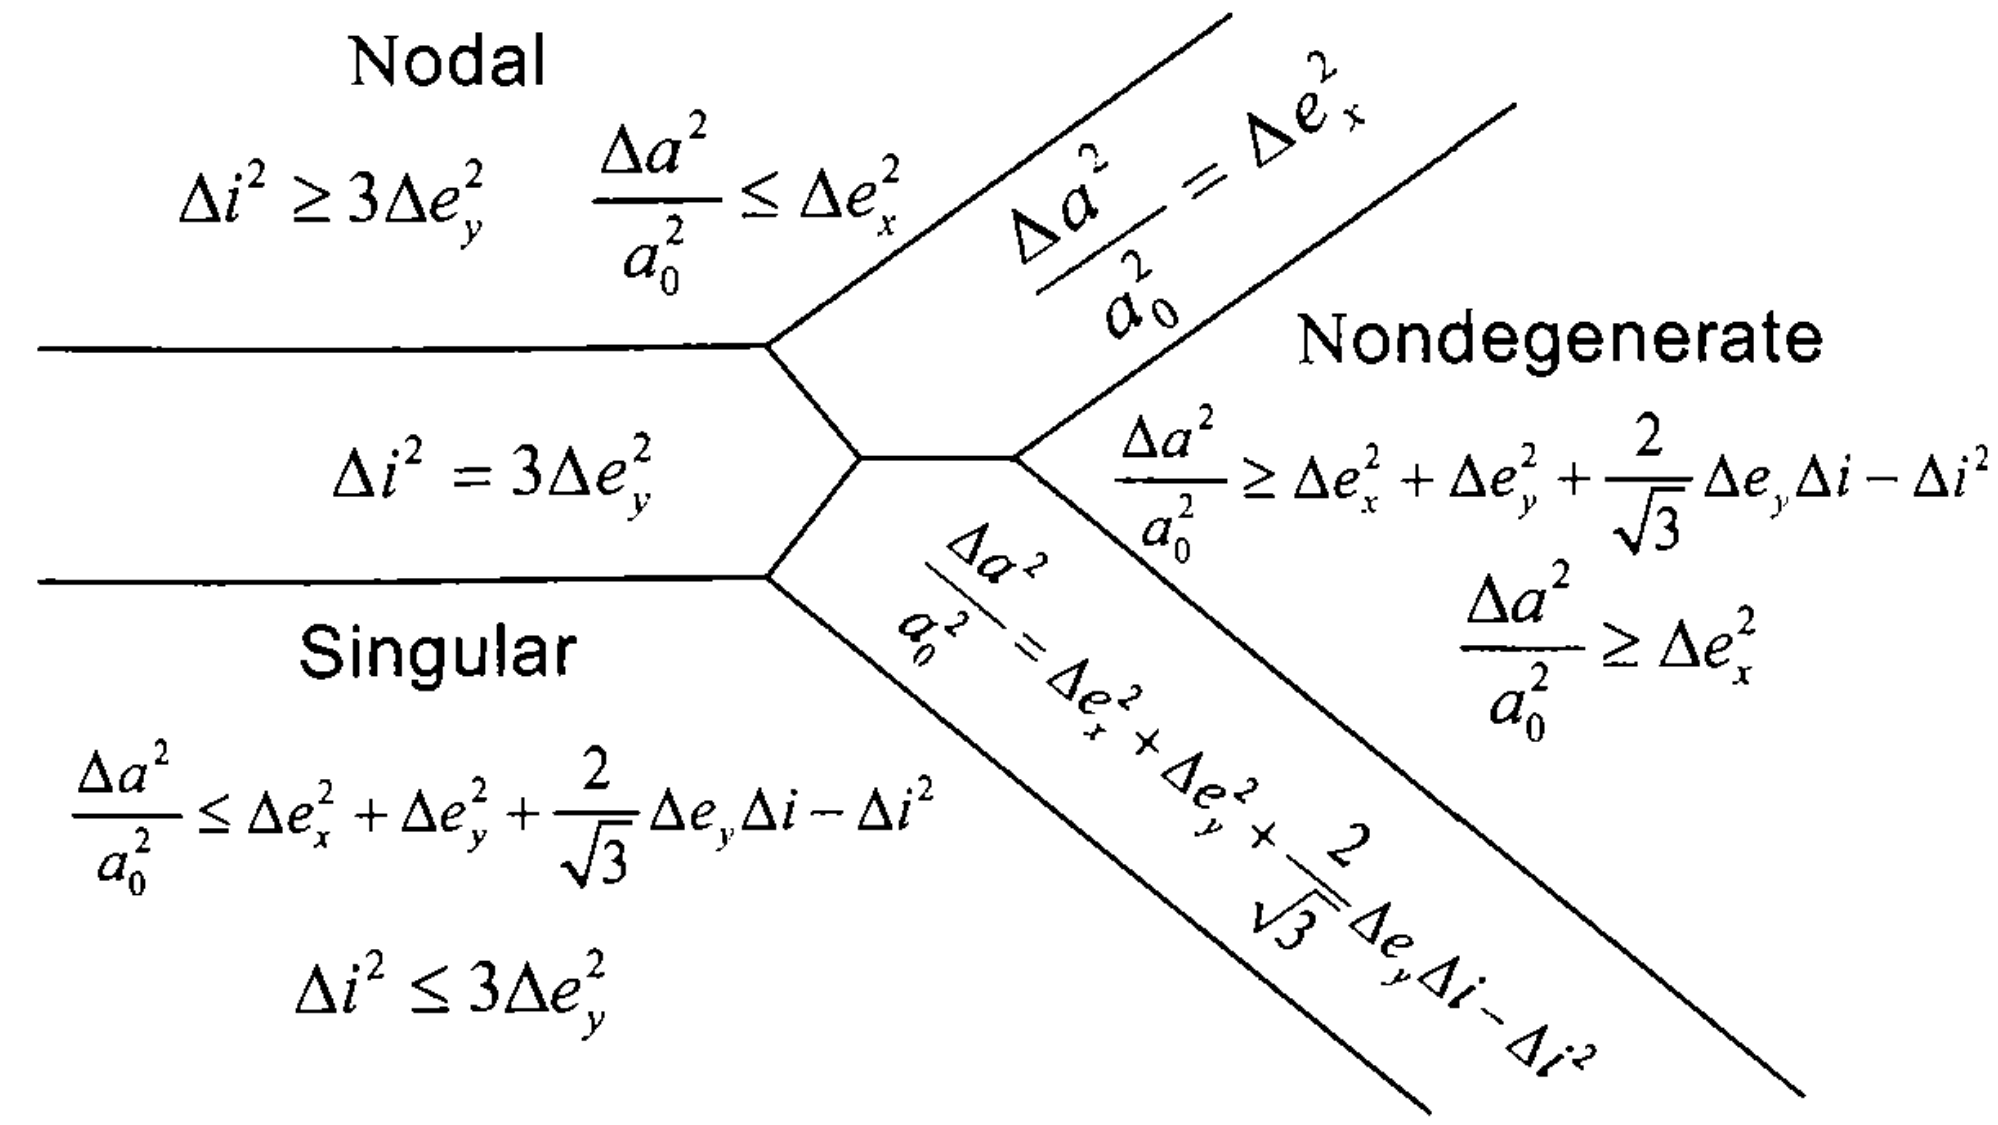
\includegraphics[height=0.7\textheight,keepaspectratio]{images/5/types.png}
\end{center}
\end{frame}

\begin{frame}{Узловой случай}
\begin{columns}[T,onlytextwidth]
  % левая колонка
  \begin{column}{0.49\textwidth}
    Область существования узлового решения:
    \begin{equation*}
    \begin{cases}
        \Delta i^2 \geq 3\Delta e_y^2, \\
        \Delta a^2 \leq \Delta e_x^2.
    \end{cases}
    \end{equation*}
    Если $\Delta e_x = 0$, то решение будет выглядеть так:
    \begin{gather*}
        \Delta V_{t1} = \Delta V_{t2} = 0, \\
        \Delta V_{r1} = - \frac{\Delta e_y}{2} V_0, \quad \Delta V_{z1} = \frac{\Delta i}{2} V_0, \\
        \Delta V_{r2} = \frac{\Delta e_y}{2} V_0, \quad \Delta V_{z2} = - \frac{\Delta i}{2} V_0,
    \end{gather*}
  \end{column}

  % правая колонка
  \begin{column}{0.49\textwidth}
    Оптимальное двухимпульсное решение в общем случае:
    \begin{align*}
        \Delta V_{t1} &= \frac{1}{4} (\Delta a + \Delta e_x) V_0, \\
        \Delta V_{r1} &= -\frac{1}{2} (\Delta a + \Delta e_x) \frac{\Delta e_y}{\Delta e_x} V_0, \\
        \Delta V_{z1} &= \frac{1}{2} (\Delta a + \Delta e_x) \frac{\Delta i}{\Delta e_x} V_0, \\
        \Delta V_{t2} &= \frac{1}{4} (\Delta a - \Delta e_x) V_0, \\
        \Delta V_{r2} &= -\frac{1}{2} (\Delta a - \Delta e_x) \frac{\Delta e_y}{\Delta e_x} V_0, \\
        \Delta V_{z2} &= \frac{1}{2} (\Delta a - \Delta e_x) \frac{\Delta i}{\Delta e_x} V_0.
    \end{align*}
  \end{column}
\end{columns}
\end{frame}

\begin{frame}{Невырожденный случай}
Область существования невырожденного решения:
\begin{equation*}
\begin{cases}
    \Delta a^2 \geq \Delta e_x^2 + \Delta e_y^2 + \frac{2}{\sqrt{3}} \Delta e_y \Delta i - \Delta i^2, \\
    \Delta a^2 \geq \Delta e_x^2.
\end{cases}
\end{equation*}
Суммарная характеристическая скорость для невырожденного случая задаётся выражением:
\begin{equation*}
    \Delta V = V_0 \sqrt{\frac{1}{2}} \sqrt{A + B},
\end{equation*}
где $A = \Delta i^2 + \Delta e_x^2 + \Delta e_y^2 - \frac{1}{2} \Delta a^2$, $B = \sqrt{(\Delta i^2 - \Delta e_x^2 - \Delta e_y^2 + \Delta a^2)^2 + 4 \Delta i^2 \Delta e_y^2}$.
\end{frame}

\begin{frame}{Невырожденный случай}
Множители Лагранжа $\lambda_k$, $k \in \{1, 2, 3, 4, 5\}$, для каждой переменной состояния (элемента орбиты) будут являться частными производными от $\Delta V$ по соответствующей переменной. Следующие выражения впервые были получены в работе \cite{Edelbaum_1}:
\begin{align*}
    \lambda_1 &= \frac{\Delta a}{2 \Delta V} V_0^2 \left[ -\frac{1}{2} + \frac{\Delta i^2 - \Delta e_x^2 - \Delta e_y^2 + \Delta a^2}{\sqrt{(\Delta i^2 - \Delta e_x^2 - \Delta e_y^2 + \Delta a^2)^2 + 4 \Delta i^2 \Delta e_y^2}} \right], \\
    \lambda_2 &= \frac{\Delta e_y}{2 \Delta V} V_0^2 \left[ 1 + \frac{-\Delta i^2 - \Delta e_x^2 - \Delta e_y^2 + \Delta a^2}{\sqrt{(\Delta i^2 - \Delta e_x^2 - \Delta e_y^2 + \Delta a^2)^2 + 4 \Delta i^2 \Delta e_y^2}} \right], \\
    \lambda_3 &= \frac{\Delta e_x}{2 \Delta V} V_0^2 \left[ 1 + \frac{\Delta i^2 - \Delta e_x^2 - \Delta e_y^2 + \Delta a^2}{\sqrt{(\Delta i^2 - \Delta e_x^2 - \Delta e_y^2 + \Delta a^2)^2 + 4 \Delta i^2 \Delta e_y^2}} \right], \\
    \lambda_4 &= \frac{-\Delta e_y}{2 \Delta V} V_0^2 \left[ \frac{2 \Delta i \Delta e_y}{\sqrt{(\Delta i^2 - \Delta e_x^2 - \Delta e_y^2 + \Delta a^2)^2 + 4 \Delta i^2 \Delta e_y^2}} \right], \\
    \lambda_5 &= \frac{\Delta i}{2 \Delta V} V_0^2  \left[ 1 + \frac{\Delta i^2 - \Delta e_x^2 + \Delta e_y^2 + \Delta a^2}{\sqrt{(\Delta i^2 - \Delta e_x^2 - \Delta e_y^2 + \Delta a^2)^2 + 4 \Delta i^2 \Delta e_y^2}} \right].
\end{align*}
\end{frame}

\begin{frame}{Невырожденный случай}
Введём вспомогательный угол $\theta_0$ и определим углы приложения импульсов скорости:
\begin{gather*}
    \tan \theta_0 = \frac{\lambda_2}{\lambda_3}, \\
    \cos (\varphi_1 - \theta_0) = \frac{4 \lambda_1 \left( \sqrt{\lambda_2^2 + \lambda_3^2} \right)^3}{(\lambda_3 \lambda_4 - \lambda_2 \lambda_5)^2 - 3 \left( \lambda_2^2 + \lambda_3^2 \right)^2}, \\
    \varphi_2 = 2\theta_0 - \varphi_1.
\end{gather*}

Выпишем выражения для координат базис-вектора:
\begin{align*}
    \lambda &= - \lambda_2 \cos \varphi_1 + \lambda_3 \sin \varphi_1, \\
    \mu &= 2 \lambda_1 + 2 \lambda_2 \sin \varphi_1 + 2 \lambda_3 \cos \varphi_1, \\
    \nu &= \lambda_4 \sin \varphi_1 + \lambda_5 \cos \varphi_1.
\end{align*}
Впервые они были получены Лоуденом в работе \cite{Lawden_all} и приведены к этому виду Эдельбаумом в \cite{Edelbaum_1}.
\end{frame}

\begin{frame}{Невырожденный случай}
Теперь приведём окончательные выражения для проекций импульсов скорости:
\begin{gather*}
    \Delta V_1 = \frac{\lambda_2 \Delta V}{\lambda_2 - \lambda_1}, \quad \Delta V_2 = \frac{\lambda_1 \Delta V}{\lambda_1 - \lambda_2}, \\
    \Delta V_{t1} = \Delta V_1 \mu, \quad \Delta V_{r1} = \Delta V_1 \lambda, \quad \Delta V_{z1} = \Delta V_1 \nu, \\
    \Delta V_{t2} = \Delta V_2 \mu, \quad \Delta V_{r2} = \Delta V_2 \lambda, \quad \Delta V_{z2} = -\Delta V_2 \nu.
\end{gather*}

Решение выше может претерпевать вырождения, если $\Delta e_x = \Delta e_y = 0$. В таком случае предлагается воспользоваться следующими выражениями:
\begin{gather*}
    \Delta V_{r1} = \Delta V_{r2} = 0, \\
    \Delta V_{t1} = \frac{\Delta a}{4} V_0, \quad \Delta V_{z1} = \frac{\Delta i}{2} V_0, \\
    \Delta V_{t2} = \frac{\Delta a}{4} V_0, \quad \Delta V_{z2} = - \frac{\Delta i}{2} V_0,
\end{gather*}
Точки приложения для этого решения находятся на линии пересечения плоскостей орбит и разнесены на $180^{\circ}$.
\end{frame}

\begin{frame}{Особый случай}
Область существования особого решения:
\begin{equation}
\begin{cases}
    \Delta a^2 \leq \Delta e_x^2 + \Delta e_y^2 + \frac{2}{\sqrt{3}} \Delta e_y \Delta i - \Delta i^2, \\
    \Delta i^2 \leq 3\Delta e_y^2.
\end{cases}
\end{equation}
Получить аналитическое решение двухимпульсной задачи оптимального перехода в этом случае не представляется возможным. Поэтому воспользуемся четырёхимпульсным решением. Его выбор был обусловлен простотой реализации и возможностью разделения импульсов по направлению коррекции орбиты: в плоскости и в боковом направлении.

Первые два импульса будут отвечать за коррекцию плоскости орбиты, а потому будут иметь лишь боковые компоненты:
\begin{equation}
    \Delta V_{z1} = \frac{\Delta i}{2} V_0, \quad \Delta V_{z2} = - \frac{\Delta i}{2} V_0.
\end{equation}
Их точки приложения должны находиться на линии пересечения плоскостей орбит с интервалом в $180^{\circ}$. После этого воспользуемся уже описанными алгоритмами для компланарных переходов, что и завершит решение этой задачи.
\end{frame}

\begin{frame}{Зависимость ошибки маневрирования}
\begin{center}
    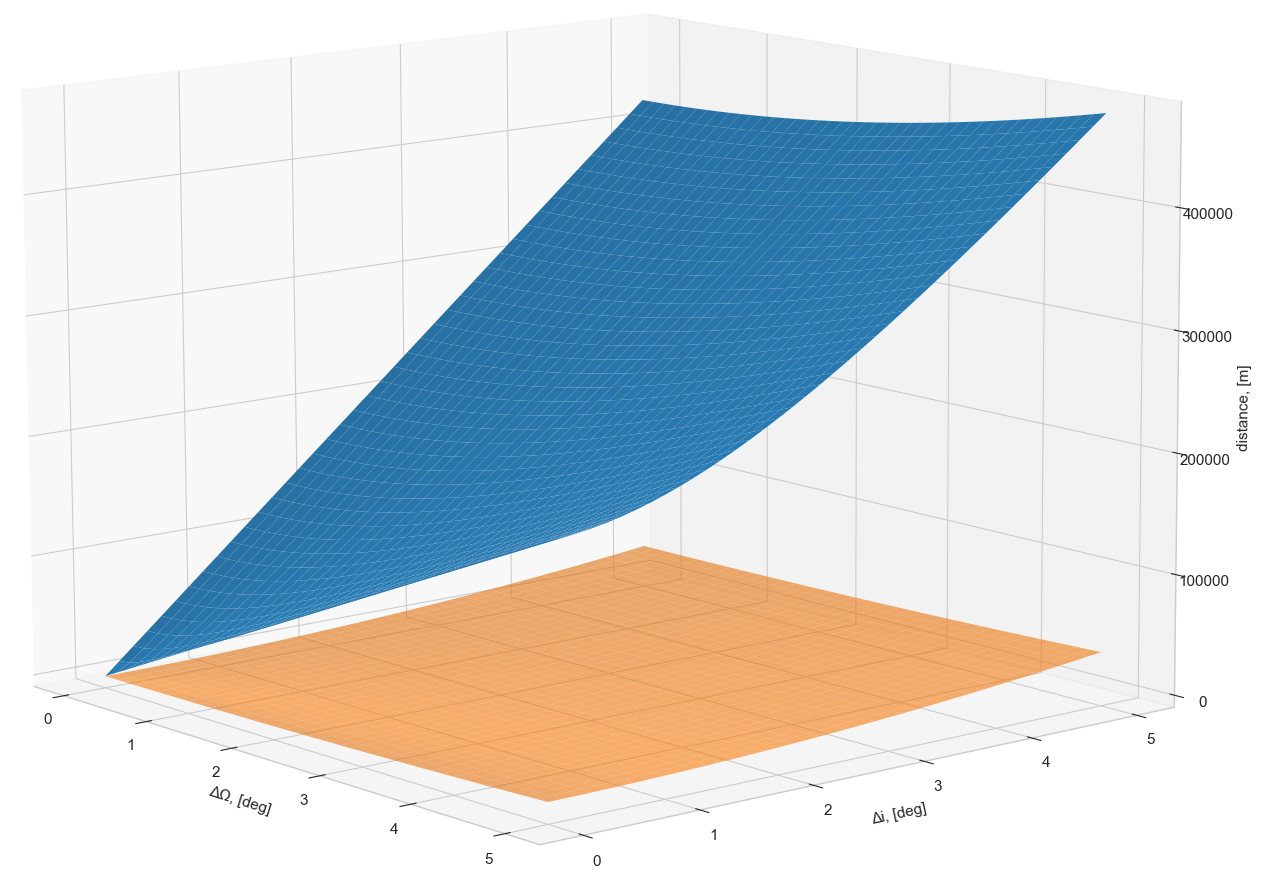
\includegraphics[height=0.75\textheight,keepaspectratio]{images/5/dist_init_final.png}
\end{center}
\end{frame}

\begin{frame}{Зависимость ошибки маневрирования}
\begin{center}
    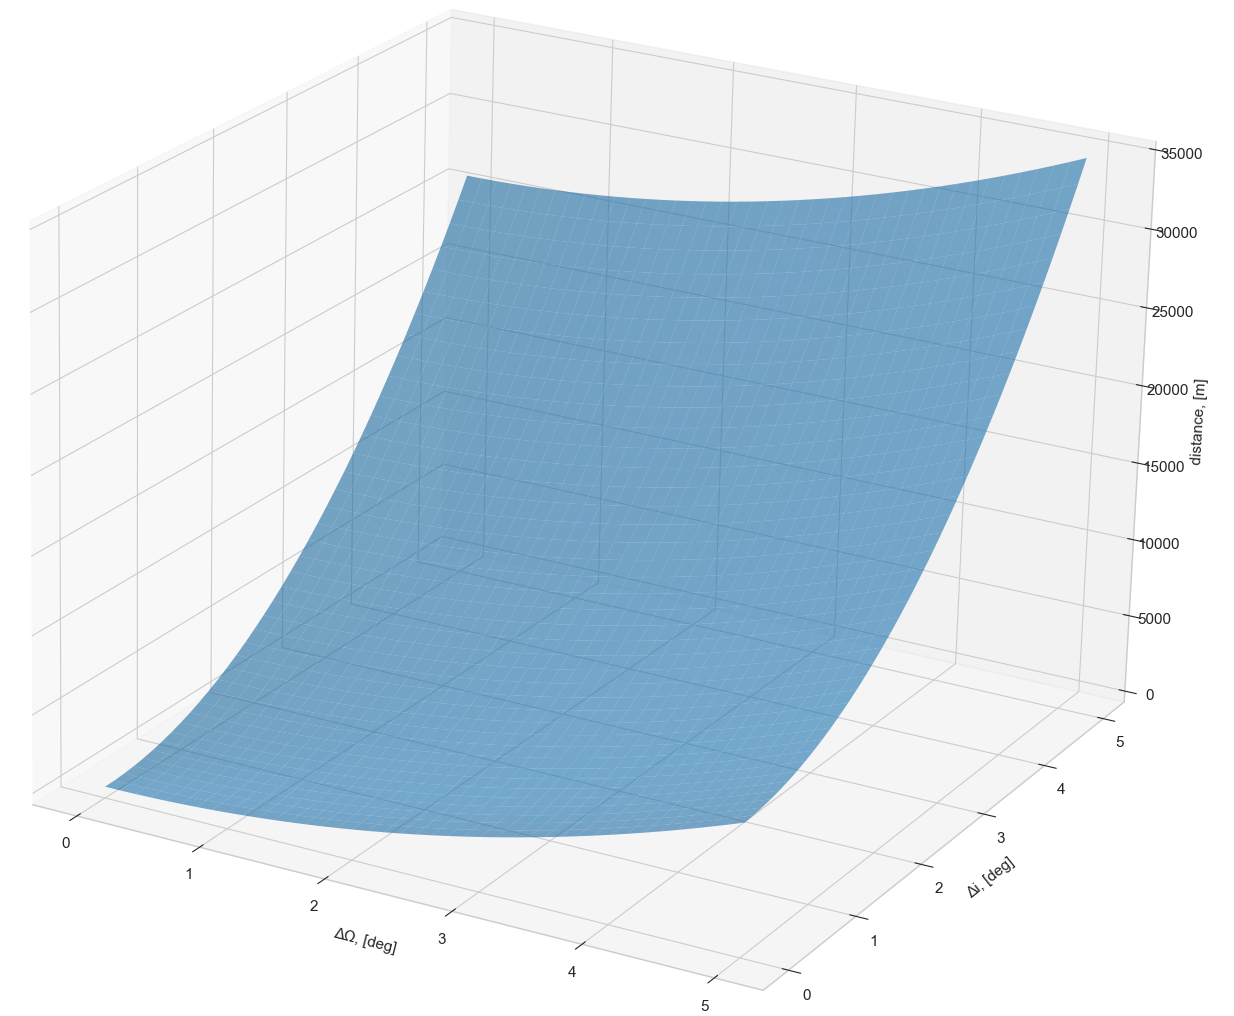
\includegraphics[height=0.75\textheight,keepaspectratio]{images/5/dist_final.png}
\end{center}
\end{frame}

\begin{frame}{"Стоимость" изменения элементов орбиты}
\begin{center}
    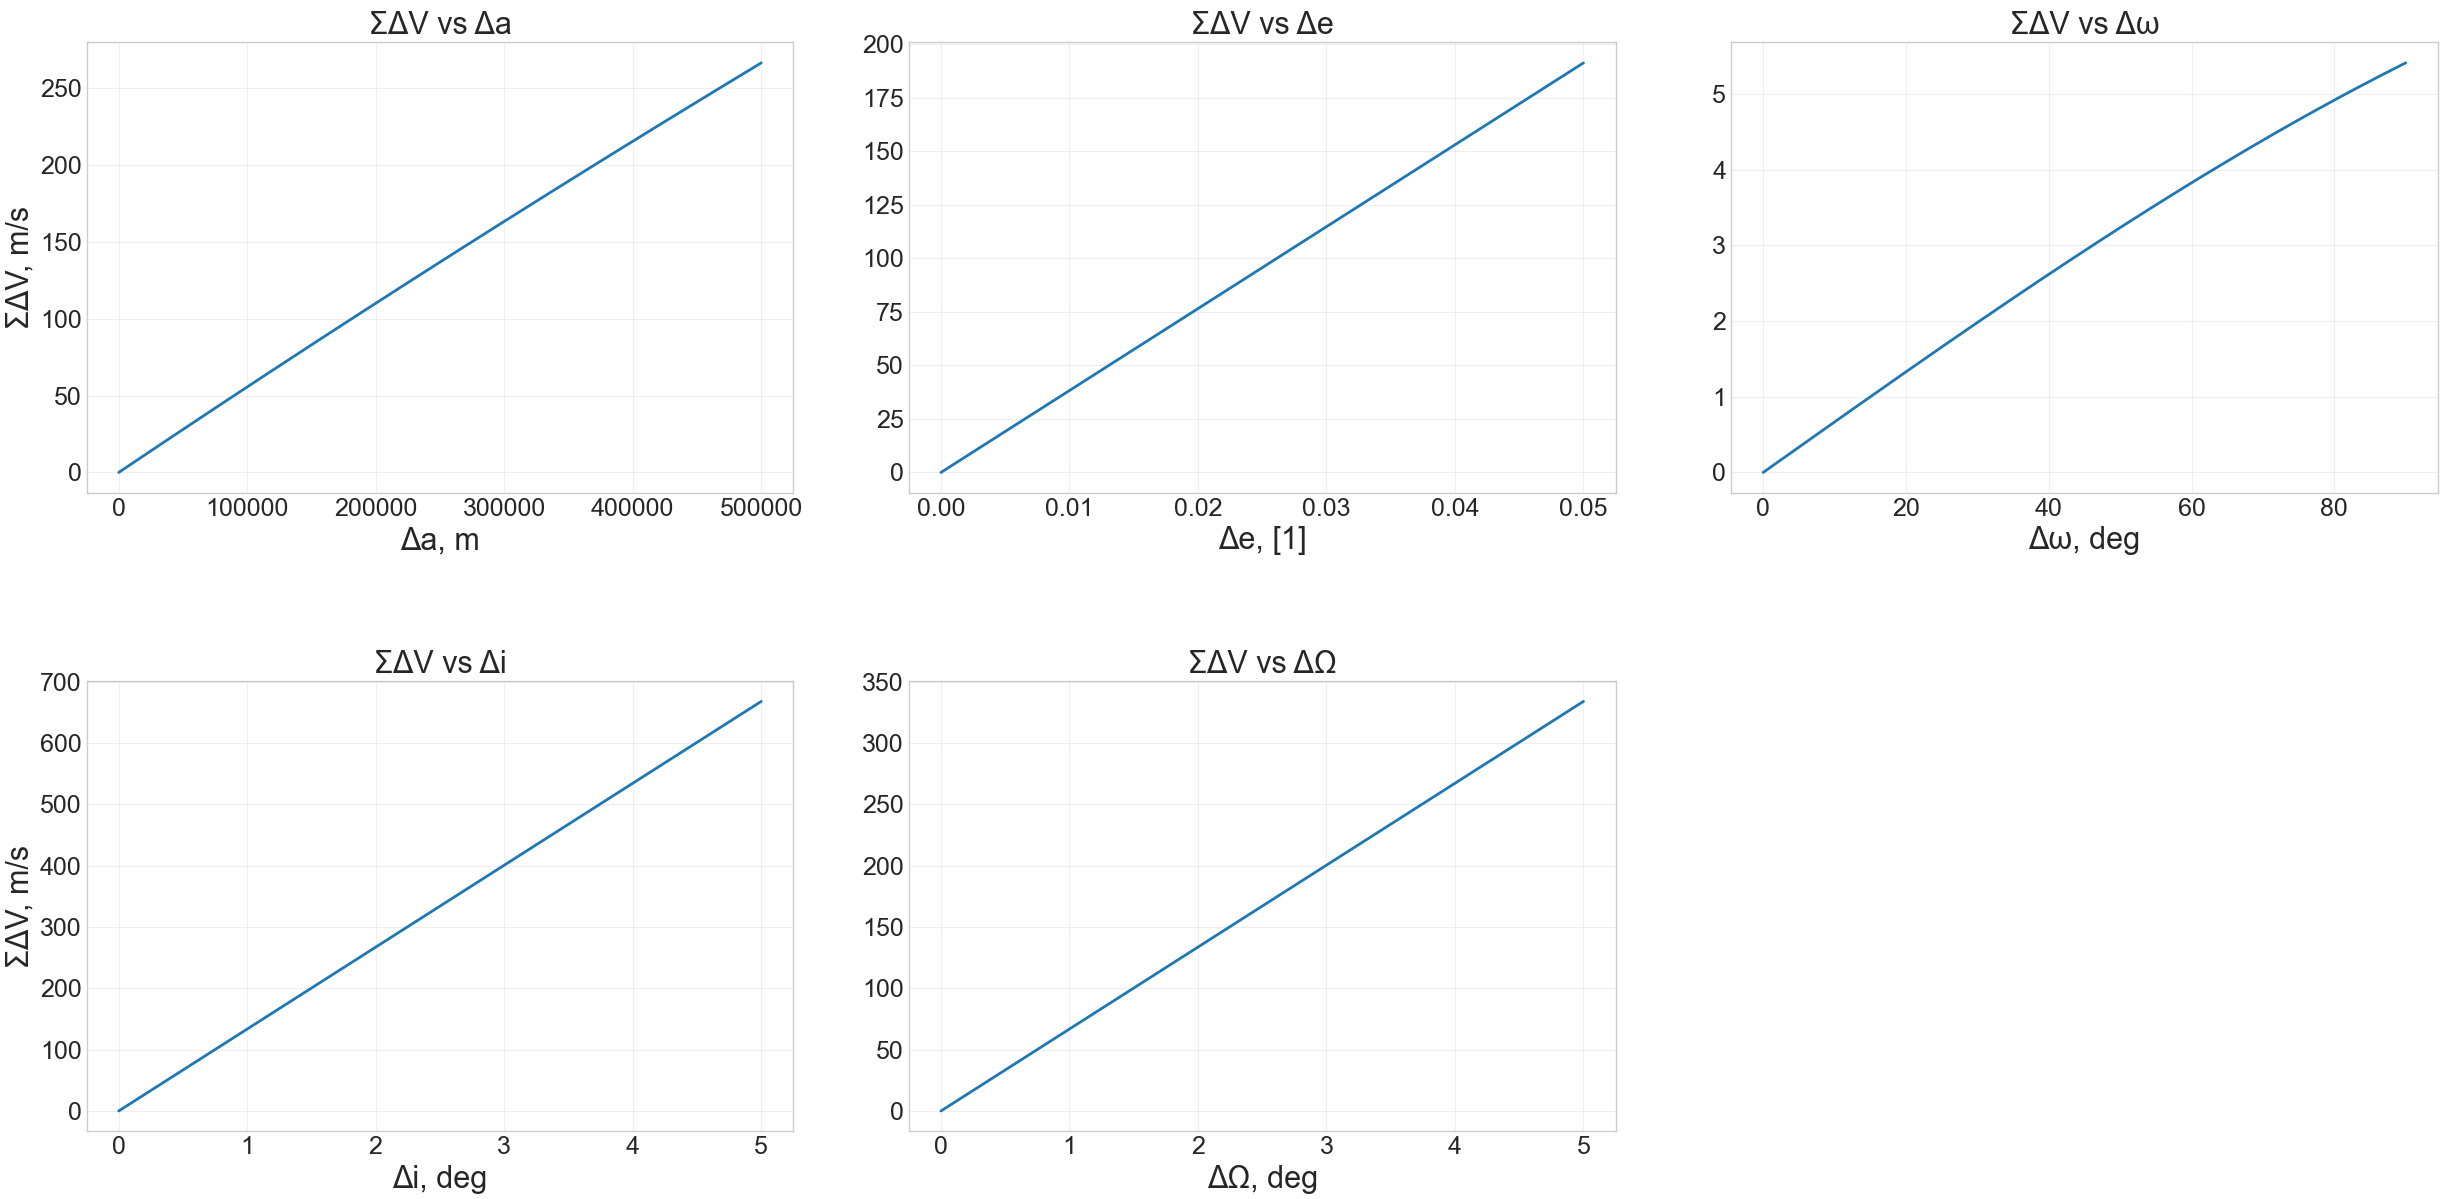
\includegraphics[height=0.6\textheight,keepaspectratio]{images/5/dv_vs_dE.png}
\end{center}
\end{frame}

\begin{frame}{Узловой случай}
\begin{center}
    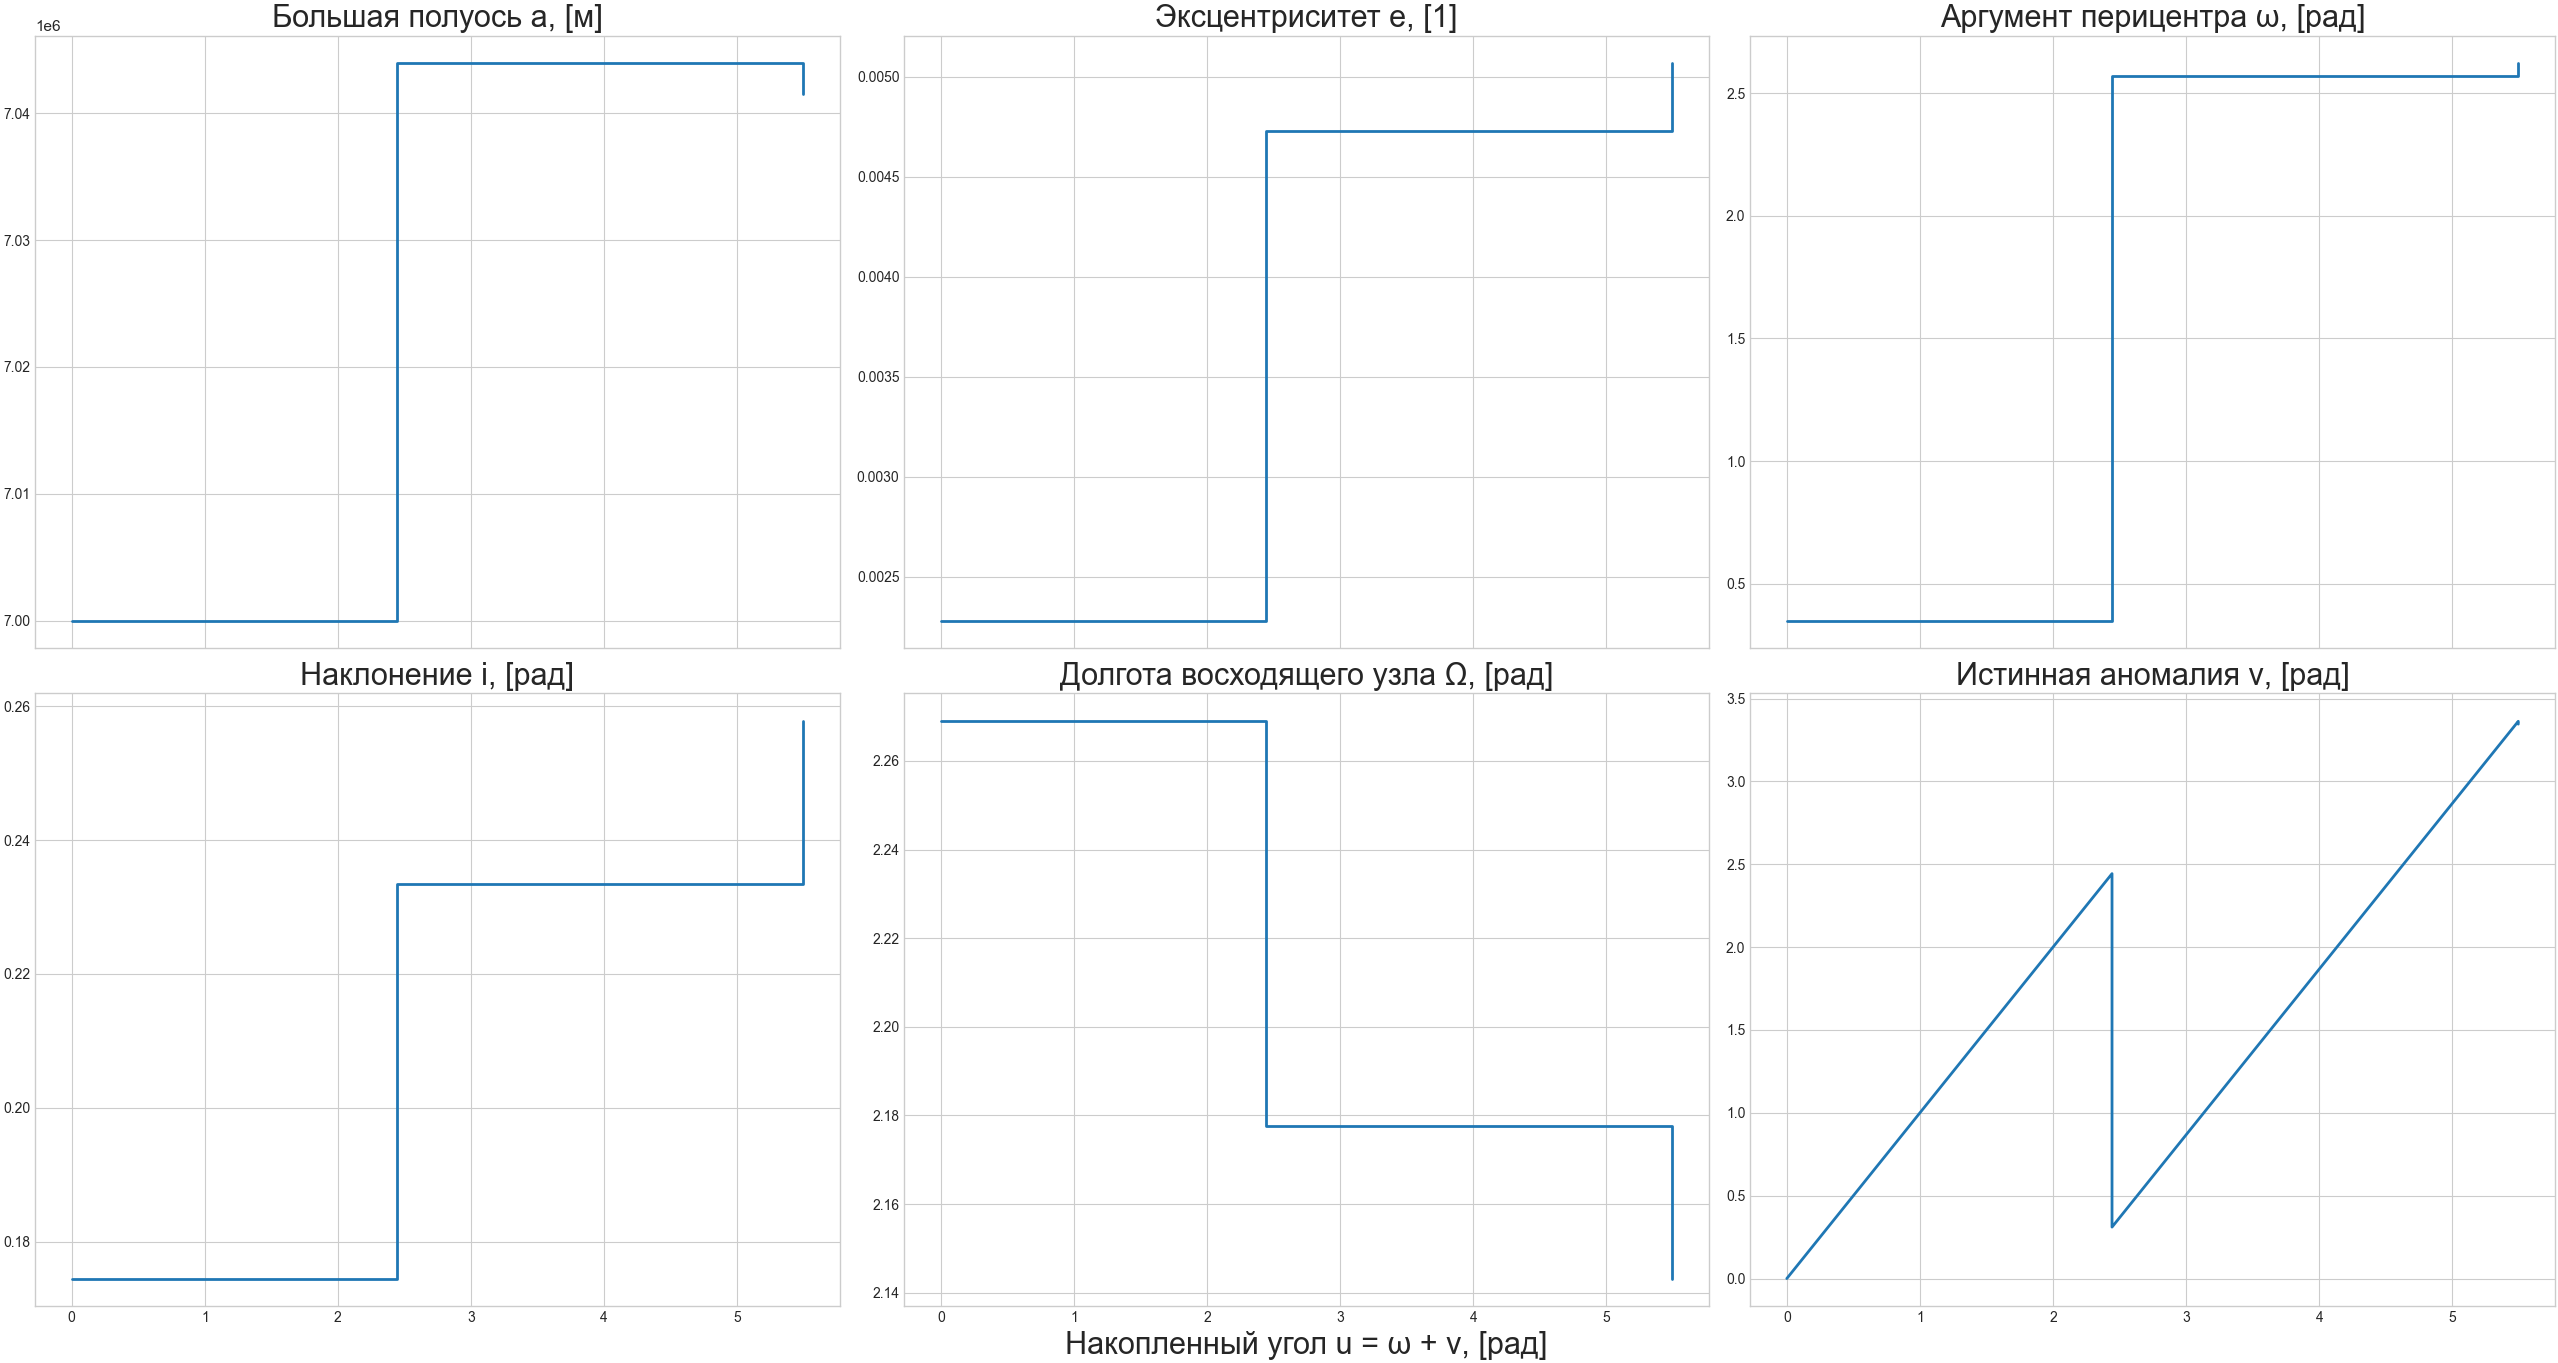
\includegraphics[height=0.7\textheight,keepaspectratio]{images/5/nodal.png}
\end{center}
\end{frame}

\begin{frame}{Невырожденный случай}
\begin{center}
    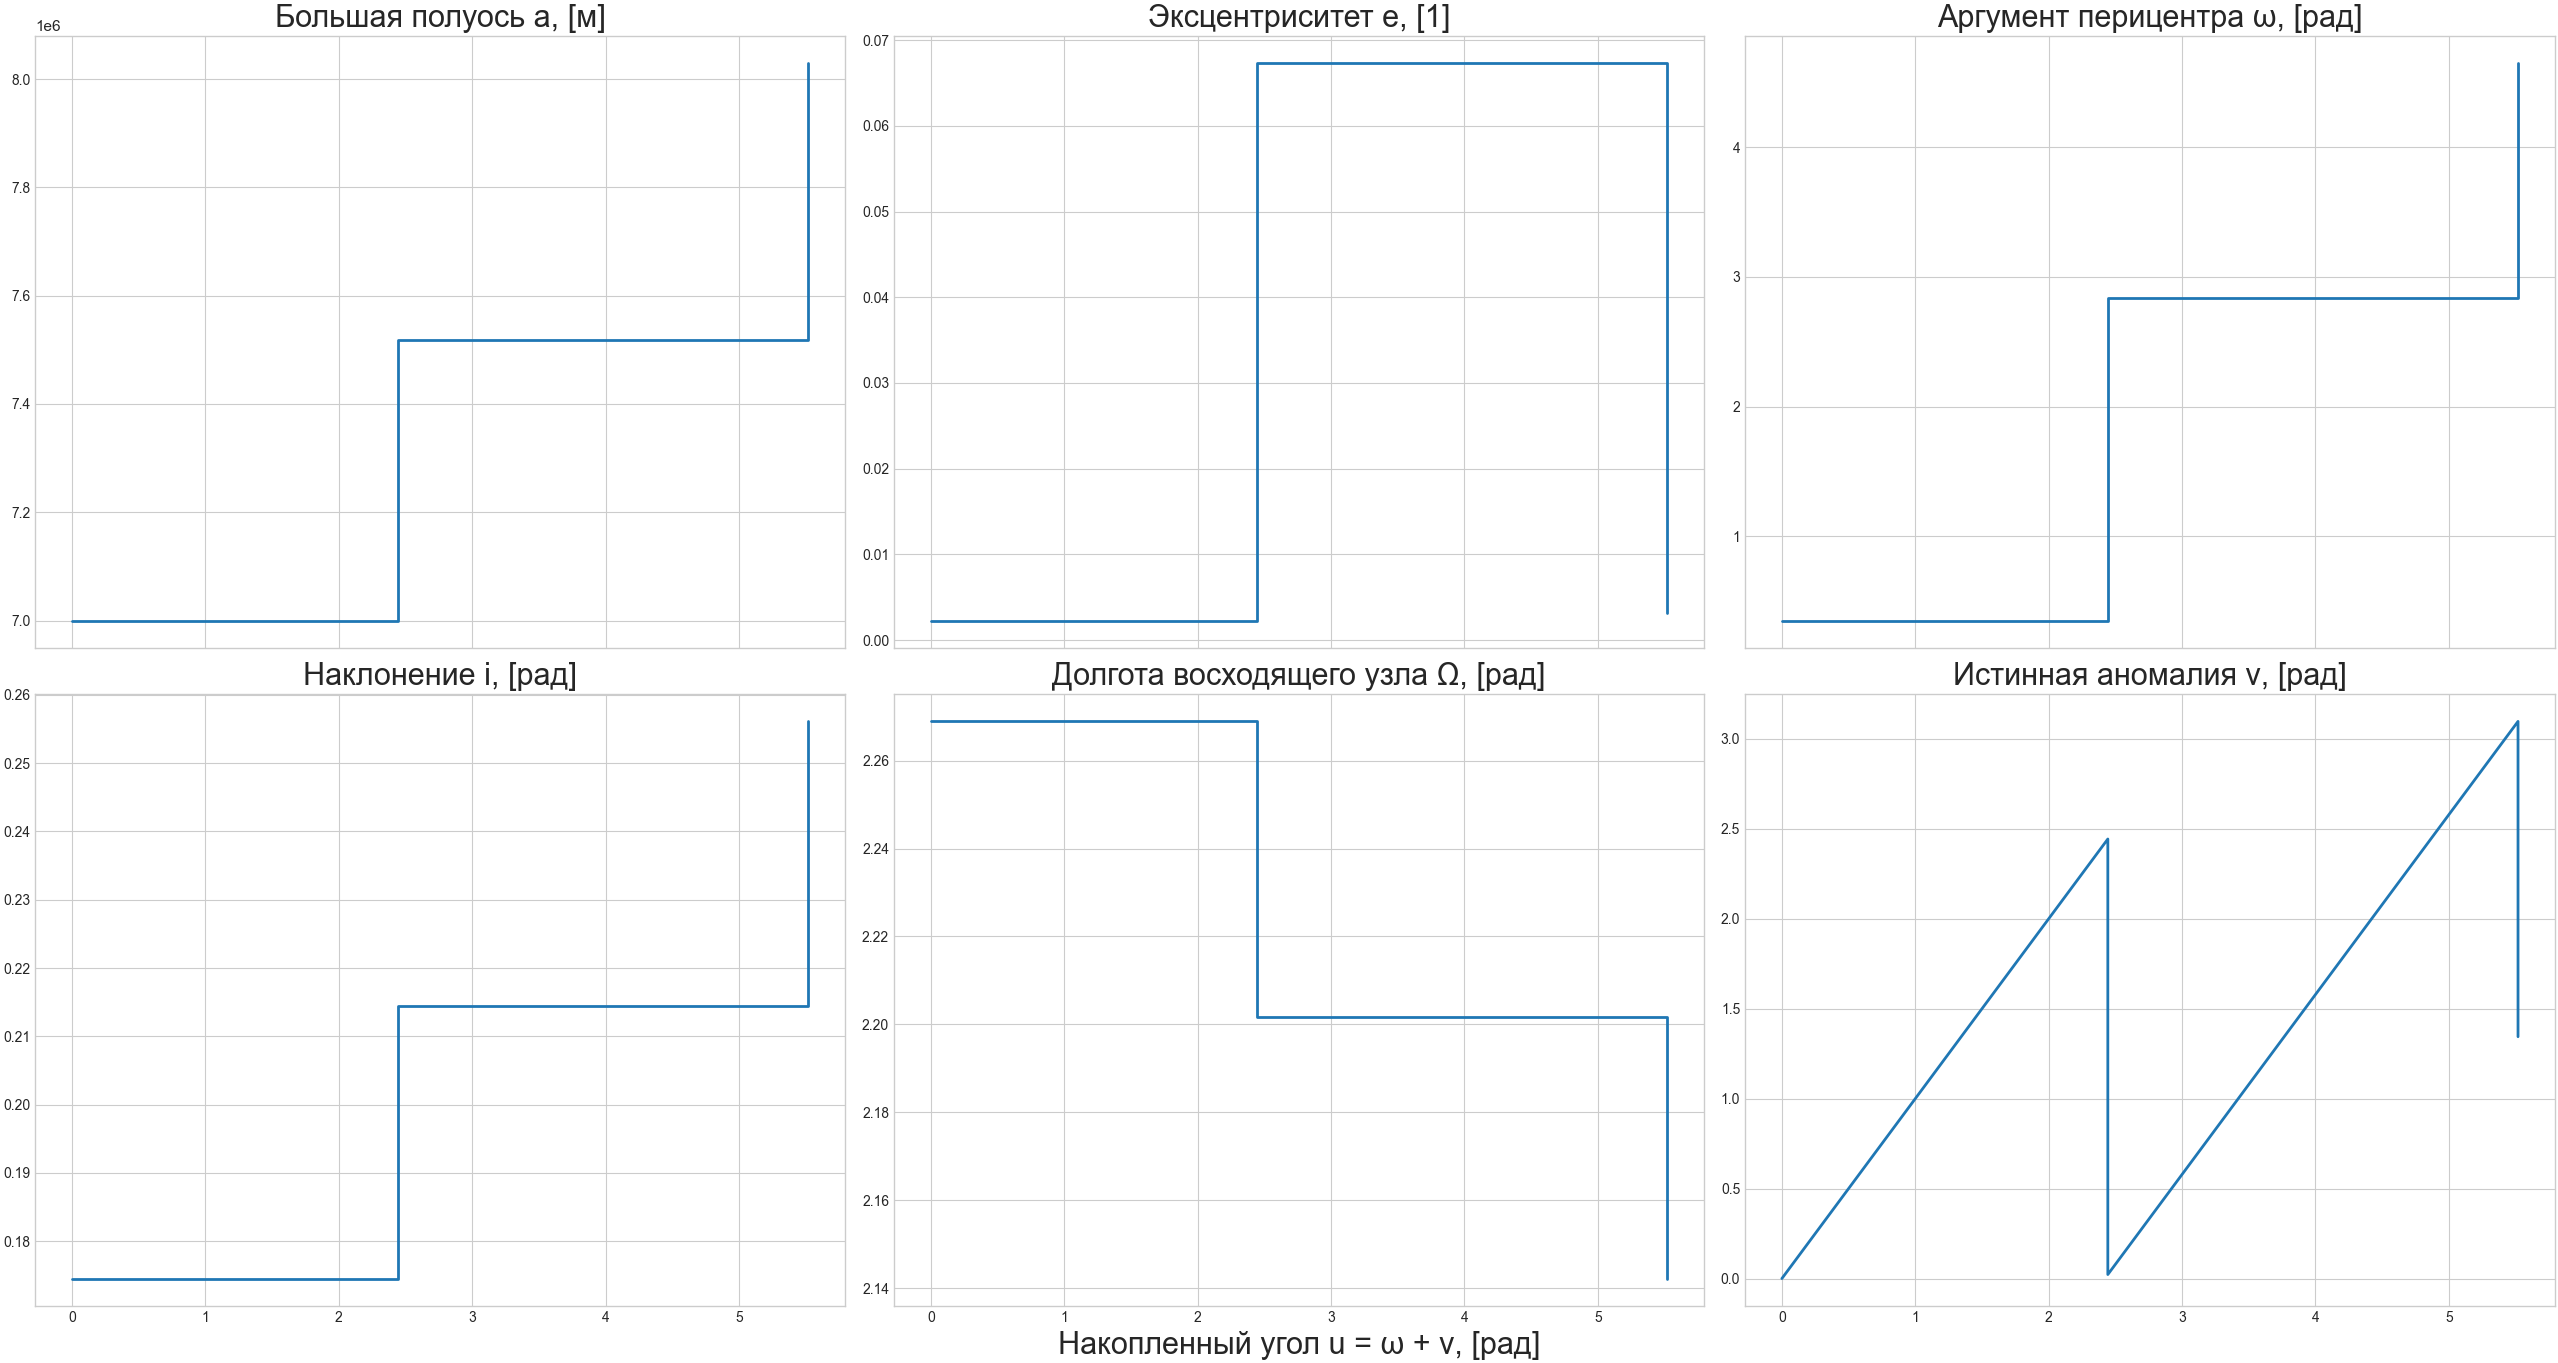
\includegraphics[height=0.7\textheight,keepaspectratio]{images/5/nondegenerate.png}
\end{center}
\end{frame}

\begin{frame}{Особый случай}
\begin{center}
    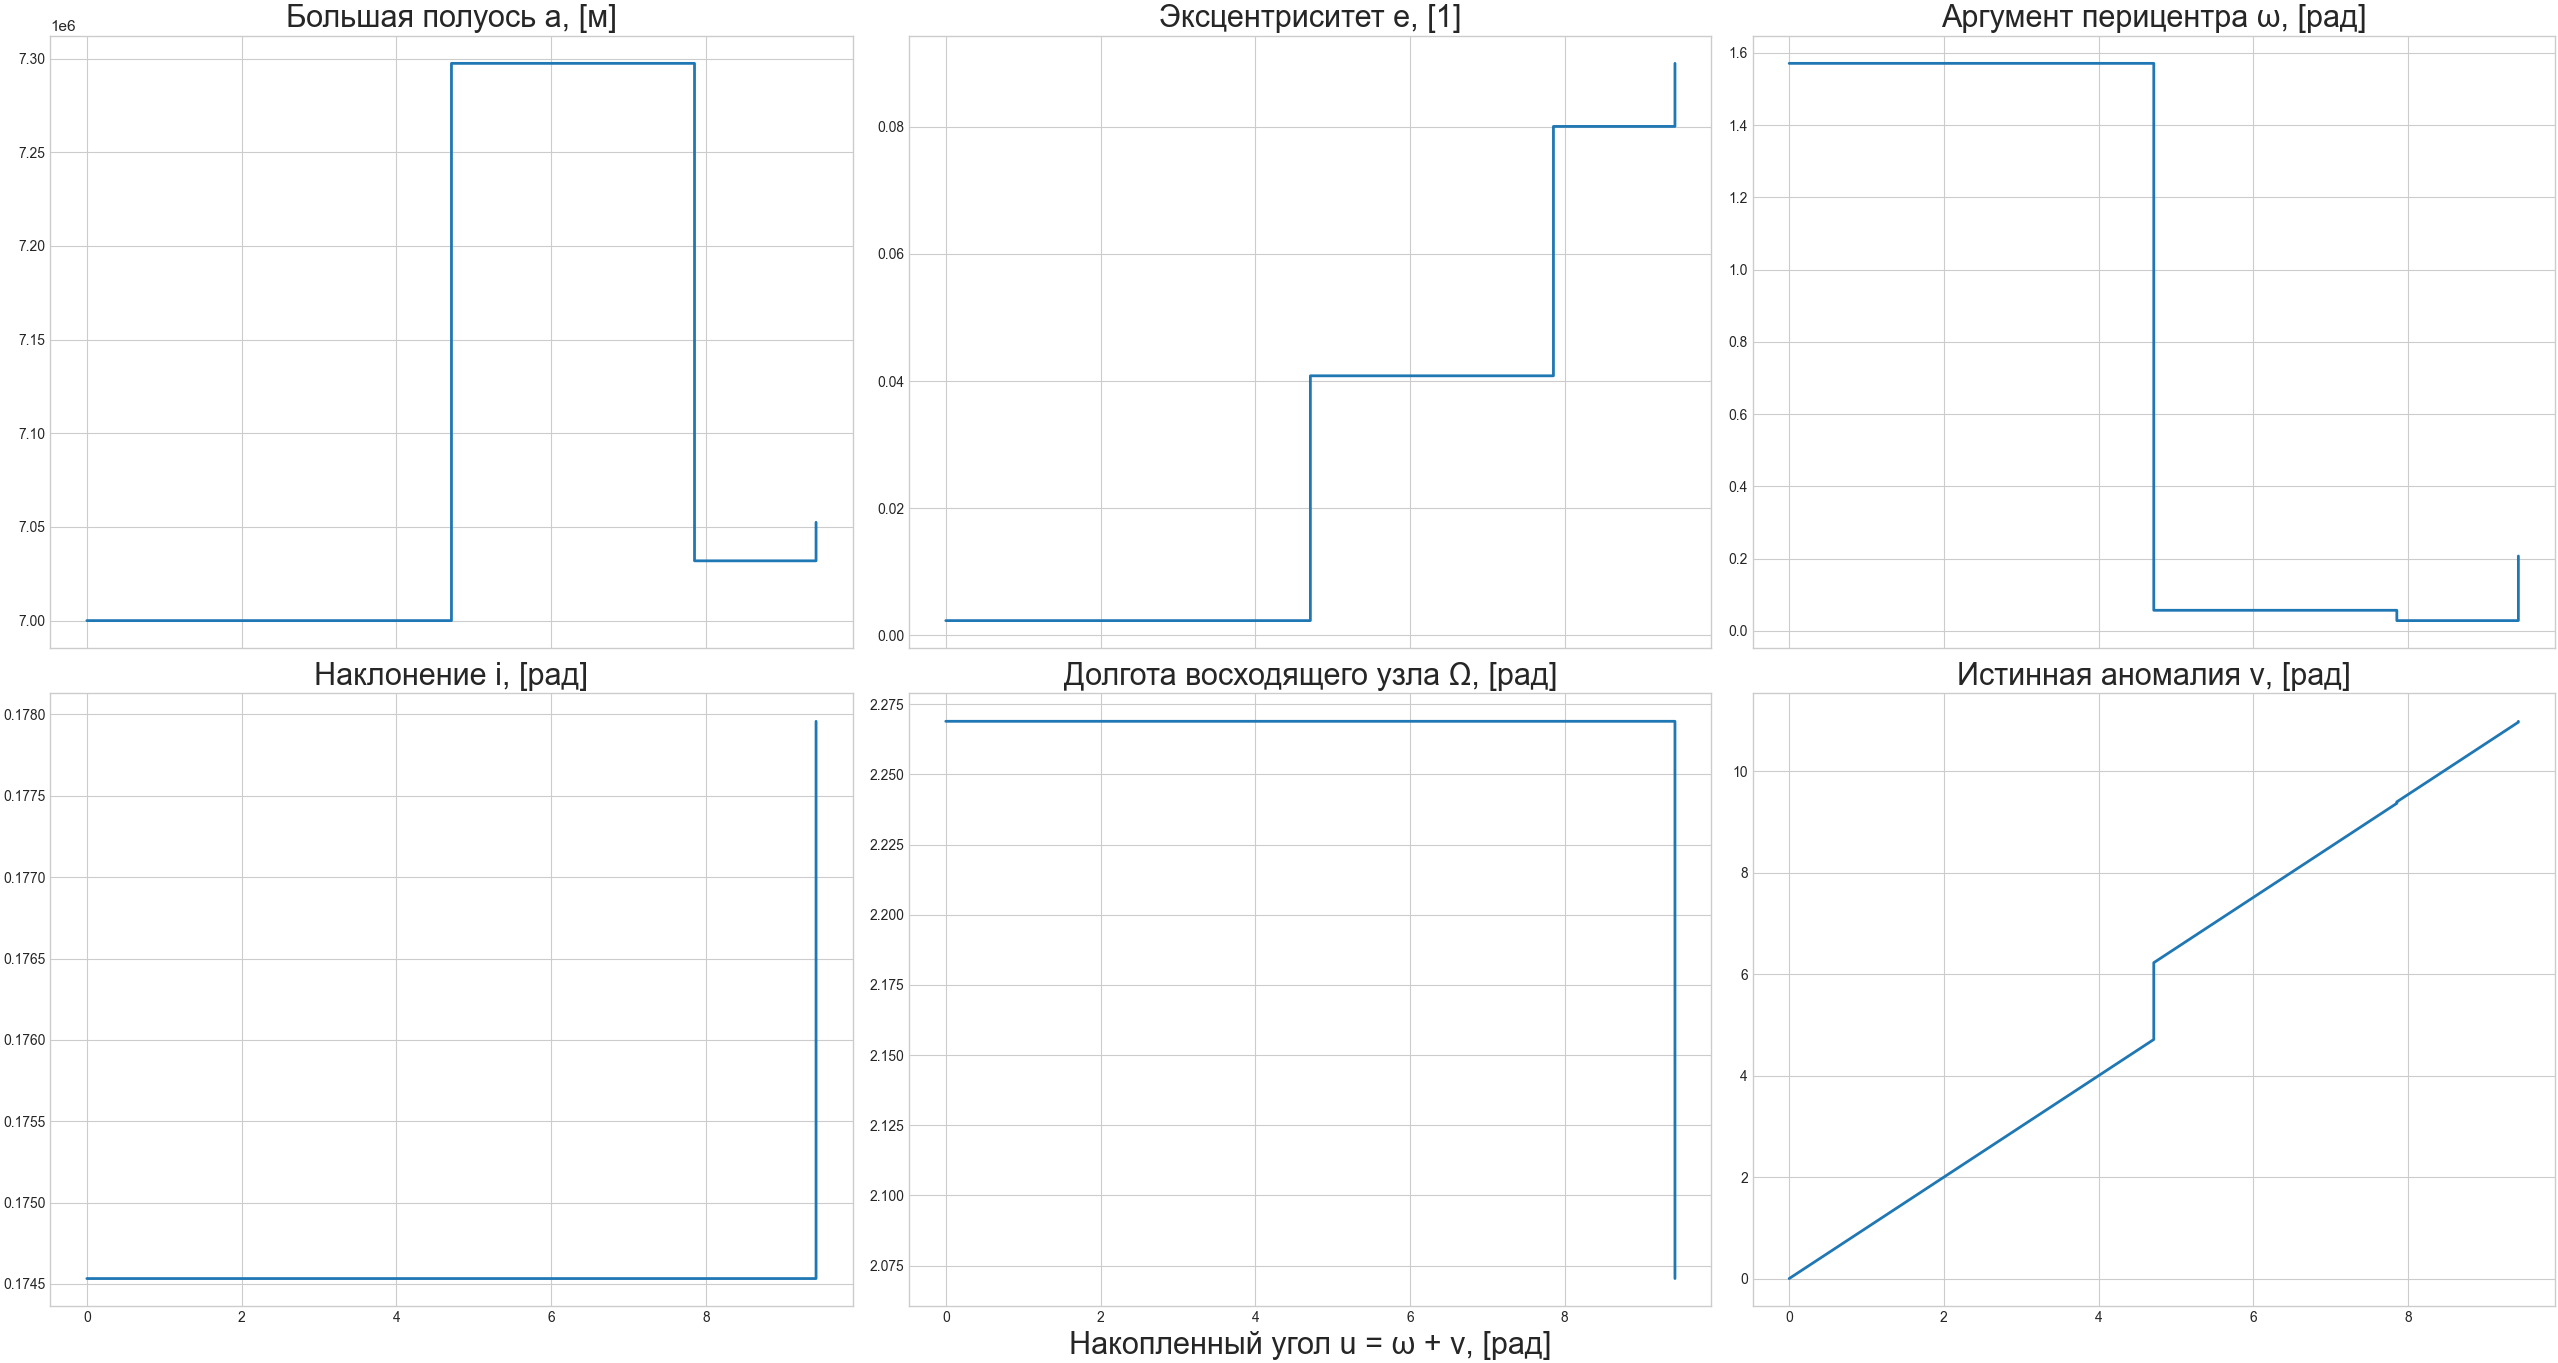
\includegraphics[height=0.7\textheight,keepaspectratio]{images/5/singular.png}
\end{center}
\end{frame}

\begin{frame}{Итоги}
Мы рассмотрели решение задачи перехода в линейном приближении. Такое приближение позволяет:
\begin{itemize}
    \item Получить \textbf{аналитические} выражения для \textbf{оптимальных} алгоритмов перехода;
    \item Исследовать характер влияния мгновенных импульсов на изменение орбитальных элементов и дальнейшую эволюцию орбиты.
\end{itemize}
Минусы полученного решения:
\begin{itemize}
    \item Может давать большую ошибку;
    \item Не учитывает никакие возмущающие факторы;
    \item Оптимальным решение будет являться только в существующей постановке задачи: точечный потенциал, мгновенные импульсы.
\end{itemize}
\end{frame}

\begin{frame}[allowframebreaks]{Источники}
  \begin{thebibliography}{9}

    \bibitem{Southworth_Hawkins}
    Southworth R. B., Hawkins G. S. Statistics of meteor streams //Smith. Contrib. Astrophys.―1963.―7.―P. – 1963. – С. 261-285.
  
    \bibitem{Kholshevnikov}
    Kholshevnikov K. V., Vassiliev N. N. Natural metrics in the spaces of elliptic orbits //Celestial Mechanics and Dynamical Astronomy. – 2004. – Т. 89. – С. 119-125.

    \bibitem{Edelbaum_1}
    Edelbaum T. N., Gobetz F. W., Washington M. Minimum-impulse time-free transfer between elliptic orbits. – 1966. – №. NASA-CR-636.

    \bibitem{Lawden_all}
    Лоуден Д. Ф. Оптимальные траектории для космической навигации. – 1966.
    
  \end{thebibliography}
\end{frame}

\end{document}